\chapter{AdaptaMaterialEscolar 2.0}
\label{cap:AdaptaMaterialEscolar2.0}
En este capítulo explicaremos la obtención de requisitos y cómo se han clasificado en la Sección \ref{cap:requisitos}. También se describirá el diseño realizado por cada integrante de la aplicación para la iteración competitiva y el diseño final de las funcionalidades en la Sección \ref{disenyoDeLaAplicacion}.


\section{Requisitos}
\label{cap:requisitos}

Lo primero que hicimos fue analizar la memoria de AdaptaMaterialEscolar 1.0 \citep*{AdaptaMaterialEscolar1.0}extrayendo las funcionalidades que faltaban por implementar y los resultados de la evaluación que se realizó. Tras este análisis hemos decidido agrupar las nuevas funcionalidades según los datos sobre los que trabajan y las acciones que realizan.

De esta forma han surgido las siguientes agrupaciones: formato (funcionalidades que tienen relación con el estilo o la estructura del documento), ejercicios (funcionalidades relacionadas con la creación de actividades) y auxiliar (resto de funcionalidades que no pertenecen a formato o a ejercicios). Quedan así las funcionalidades agrupadas de la siguiente manera:
\\

\begin{itemize}
  \item Funcionalidades relacionadas con el formato:
        \begin{itemize}
          \item Añadir encabezado al texto: El usuario eligirá un encabezado que se añadirá al documento de trabajo.
          \item Añadir un tipo de fuente escolar: Incluir en los tipos de fuentes la escolar. Dicha fuente se refleja en la Figura \ref{escolar}.
                \begin{figure}[ht!]
                  \centering
                  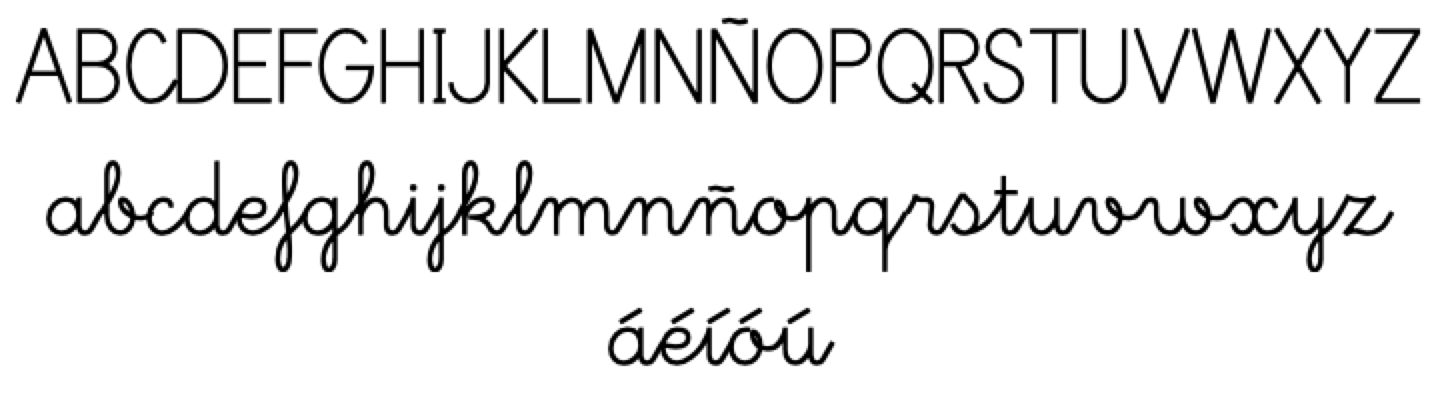
\includegraphics[scale=0.3]{AdaptaMaterialEscolar/FunteEscolar.png}
                  \caption{Fuente escolar.}
                  \label{escolar}
                \end{figure}
          \item Añadir una leyenda de colores: Sirve para que el docente pueda poner de distintos colores distintas palabras según la categoría a la que pertecenecen, por ejemplo sustantivos en rojo y adjetivos en verde.
          \item Añadir leyenda de colores para el tema de cada asignatura: Dar la posibilidad de que cada asignatura tenga un color. Al crear un documento según la asignatura se pondrá el borde del documento del color que corresponde a dicha asignatura.
          \item Añadir cuadrícula: En vez de renglones de una única línea se podrá poner para responder a una pregunta la cuadrícula.
          \item Añadir la opción de añadir doble pauta: En vez de renglones de una única línea se podrá poner para responder a una pregunta la doble pauta.
          \item Estandarizar formato para títulos e índices del temario: Dar la opción de crear estilos para estandarizar documento de trabajo.
          \item Enumerar ejercicios de forma automática: Establecer un orden numérico para los ejercicios de forma automática según se van creando para que el usuario no se tenga que preocupar de ese aspecto.
        \end{itemize}

  \item Funcionalidades asociadas con la creación de ejercicios:
        \begin{itemize}
          \item Ejercicios de relacionar contenido mediante flechas: Generar un ejercicio para relacionar conceptos mediante flechas.
          \item Añadir ejercicios de cálculo con huecos a rellenar por el alumno: Posibilidad de introducir ejercicios de cálculo con espacios en blanco para que el alumno rellene dichos huecos con contenido adecuado.
          \item Añadir ejercicios con espacio para dibujar: Añadir amplio hueco en blanco con el fin de que el alumno pueda dibujar.
          \item Ejercicios de completar los espacios en blanco en tablas y esquemas: Dada una tabla o un esquema se establecen espacios en blanco para que el alumno los rellene con el contenido adecuado.
        \end{itemize}

  \item Funcionalidades auxiliares:
        \begin{itemize}
          \item Generar un resumen a partir de un texto.
          \item Exportar el documento a formato Word.
          \item Añadir un pictotraductor: Que permita dada una frase traducirla a pictogramas.
          \item Añadir imágenes buscando una palabra: A partir de una palabra se busca su respectiva imagen en las bases de datos de imágenes libres.
          \item Sustituir una palabra por una imagen: Dado un texto esta funcionalidad permitirá que se seleccione una palabra, se busque una imagen asociada a dicha palabra y esta se reemplazará por la imagen seleccionada.
          \item Crear una herramienta de recorte de imágenes: Tras seleccionar una imagen se dará la opción de quitar partes de la misma.
          \item Crear tablas que organicen el temario y/o las actividades, seleccionando contenido: Tras la selección de contenido por parte del usuario se creará una tabla en base a la información seleccionada, con un formato predefinido.
          \item Creación de esquemas.
        \end{itemize}

\end{itemize}


Tras haber analizado en detalle las funcionalidades anteriores hemos encontrado que varias de ellas ya están implementadas en la versión original de AdaptaMaterialEscolar y otras hemos decidido no implementarlas actualmente ya que consideramos que no tenemos la información suficiente para ello, pero las realizaremos una vez podamos reunirnos con los usuarios finales y obtener más información sobre ellas. El resto de funcionalidades son las que implementaremos en este proyecto.

Las siguientes funcionalidades son las que ya están implementadas en la versión original:
\begin{itemize}
  \item Añadir encabezado al texto: El documento de trabajo tiene una opción con una lista de encabezados para añadir uno y cuando se pulsa un encabezado el documento de trabajo convierte el formato de la letra en el del encabezado seleccionado.
  \item Enumerar ejercicios de forma automática: El documento de trabajo permite añadir listas enumeradas.
\end{itemize}
Las funcionalidades que hemos decidido descartar de momento por falta de información son las siguientes:
\begin{itemize}
  \item Añadir imágenes buscando una palabra. Partimos de que debemos usar una base de datos de imagen libre pero no tenemos la información suficiente para definir cuál sería la base de datos correcta.
  \item Sustituir una palabra por una imagen. No la realizaremos ya que no tenemos claro de dónde obtener las imágenes ni el estilo de estas.
  \item Crear una herramienta de recorte de imágenes para el texto original: No la realizaremos ya que no tenemos claro qué tipo de recorte tenía pensado el usuario.
  \item Crear tablas que organicen el temario y/o las actividades, seleccionando contenido: Descartamos dicha funcionalidad ya que no tenemos la información suficiente del formato que desea el usuario.
  \item Crear esquemas: Descartamos dicha funcionalidad ya que no tenemos la información suficiente del formato que desea el usuario.
  \item Ejercicios de completar los espacios en blanco en tablas y esquemas. Descartamos esta funcionalidad ya que depende de la funcionalidad de crear tablas y esquemas.
\end{itemize}

Por lo tanto, las funcionalidades que vamos a implementar son las que se muestran a continuación:


\begin{itemize}
  \item Generar un resumen a partir de un texto con el fin de ayudar a un alumno a comprender los elementos claves del texto de manera mas rápida.
  \item Exportar el documento a formato Word para hacer modificaciones y que el usuario pueda continuar con las modificiones del documento.
  \item Añadir un pictotraductor con el fin de trasformar un texto a su equivalente en pictogramas para que el alumno pueda adquirir nuevos conocimientos de forma más sencilla.
  \item Ejercicios de relacionar contenido mediante flechas ya que ayuda al alumno a consolidar conceptos.
  \item Añadir un tipo de fuente escolar con el fin de facilitar la lectura y la escritura al alumno.
  \item Añadir una leyenda de colores con la categoría de cada tipo con el fin de  ayudar al alumno a relacionar conceptos.
  \item  Añadir ejercicios de cálculo con huecos a rellenar por el alumno para que el alumno practique el cálculo.
  \item  Añadir ejercicios con espacio para dibujar con el fin de que el alumno pueda reflejar lo que piensa, interpreta y representa sobre algo.
  \item Añadir leyenda de colores para el tema de cada asignatura con el fin de que el alumno pueda distinguir entre las asignaturas.
  \item Añadir cuadrícula para escribir los números con el fin de facilitar los ejercicios de matemáticas.
  \item Añadir la alternativa de añadir doble pauta con el fin de que el alumno adquiera un tamaño de letra adecuado.
  \item Estandarizar formato para títulos e índices del temario con el fin de que el profesor pueda definir un estilo.

\end{itemize}

\section{Diseño de la aplicación}
\label{disenyoDeLaAplicacion}
Analizando la interfaz de AdaptaMaterialEscolar 1.0 hemos llegado a la conclusión de que la experiencia de usuario no era cómoda. Por ejemplo, obligaba a cargar un PDF y las funcionalidades se abrían en una ventana bastante pequeña. Además, la selección de colores no nos pareció la adecuada y el estilo general de la aplicación no era moderno. Por todo lo anterior decidimos rediseñar la aplicación.

Para el rediseño hemos realizado una iteración de diseño competitiva. Esta trata de la creación, por parte de cada integrante, de un nuevo diseño de la aplicación y la puesta en común de los diseños para debatir sobre qué sería lo óptimo e intuitivo para el usuario. Luego junto a las tutoras realizamos un \textit{brainstorming} basándonos en dichos diseños. Por último, construimos el diseño final de la aplicación.

A continuación, se explicará el diseño de la aplicación por parte de cada integrante y el diseño final de la aplicación.
\subsection{Diseño de los integrantes}
En esta sección se explicará los diseños creados por cada integrante junto a las imágenes de los mismos. Todos los diseños mencionados se encuentran en el Apéndice \ref{ape:disenyosindividuales}, en las secciones \ref{sec:disenyoAlvaro}, \ref{sec:disenyoDunia}, \ref{sec:disenyoAlberto}, \ref{sec:disenyoJohan}.

\subsubsection{Álvaro Gómez Sittima}
Para empezar, se diseñó la página de inicio la cual dispone de un menú superior con el logo de la aplicación a la izquierda y enlaces a las distintas páginas de la aplicación (Ayuda y Contacto) a la derecha. En la Figura \ref{fig:disenyoAlvaro01} se muestra el diseño de esta página. Este menú superior aparecerá en todas las páginas de la aplicación y se utilizará el logo de la aplicación como enlace a la página de inicio. En esta página el usuario podrá cargar un fichero PDF y utilizar un editor de documentos para poder adaptar el material del PDF. El acceso a las opciones de archivo, formato y adaptaciones se encontrarán como botones integrados en la barra de herramientas del editor de documentos. Además, se mostrarán opciones relevantes en un barra de herramientas flotante encima del texto que tenga seleccionado en el PDF o en el editor de documentos. El diseño de esta página sin un PDF cargado se puede ver en la Figura \ref{fig:disenyoAlvaro01a} y con un PDF cargado en la Figura \ref{fig:disenyoAlvaro01b}. Si el usuario pulsa el enlace de ayuda en el menú superior, este le llevará a la página de ayuda la cual dispondrá de un buscador con el que podrá buscar información sobre un tema en concreto, relacionado con el uso de la aplicación. Si no se realiza una búsqueda aparecerán todos los temas sobre los que se ofrece ayuda. Cada tema aparecerá en una tarjeta con información sobre el tema y un breve video para apoyar lo explicado en el texto.

En cuanto a las funcionalidades, se realizarón los siguientes diseños:
\begin{itemize}
  \item \textbf{Generar resumen}: En caso de que el usuario tenga texto seleccionado, cuando pulse la opción de generar resumen le saldrá una pequeña ventana encima con un campo para introducir el número de palabras del resumen y un botón para generar el resumen, llevándolo al documento de trabajo. En la Figura \ref{fig:disenyoAlvaro02} se muestra el diseño de esta funcionalidad en caso de tener texto seleccionado. En caso de no tener texto original, se abrirá una ventana aparte donde el usuario podrá escribir el texto a resumir y resumirlo.
  \item \textbf{Pictotraductor}: En caso de que el usuario tenga texto seleccionado, cuando pulse la opción de pictotraductor se traducirá automáticamente el texto a pictogramas y se llevará al documento de trabajo. Si pulsa alguno de los pictogramas generados podrá cambiarlo por otro. En la Figura \ref{fig:disenyoAlvaro03} se muestra el diseño de esta funcionalidad en caso de tener texto seleccionado. En caso de no tener texto original, se abrirá una ventana aparte donde el usuario podrá escribir el texto y traducirlo.
  \item \textbf{Definir huecos}: En caso de que el usuario tenga texto seleccionado, cuando el usuario pulse la opción de definir huecos, se llevará automáticamente el texto al documento de trabajo y el usuario podrá definir los huecos seleccionando las palabras. En la Figura \ref{fig:disenyoAlvaro04} se muestra el diseño de esta funcionalidad en caso de tener texto seleccionado. En caso de no tener texto original, se abrirá una ventana aparte donde el usuario podrá escribir el texto y definir los huecos.
  \item \textbf{Buscar pictograma}: Cuando el usuario pulse la opción de buscar pictogramas en la barra de herramientas del editor, se abrirá una ventana modal con un buscador. Al pulsar el botón de buscar, se mostrarán todos los pictogramas relacionados con el texto introducido, debajo del buscador. El usuario podrá arrastrar los pictogramas que desee al documento de trabajo. En la Figura \ref{fig:disenyoAlvaro05} se muestra el diseño de esta funcionalidad.
  \item \textbf{Ejercicio de definiciones}: Cuando el usuario pulse la opción de crear ejercicio de definiciones en la barra de herramientas del editor, se creará un recuadro en el documento de trabajo donde el usuario podrá añadir los distintos conceptos a definir y el número de renglones de cada definición. Cuando haya terminado de crear el ejercicio podrá darle al botón de aceptar para que el ejercicio se inserte en el documento de trabajo. En la Figura \ref{fig:disenyoAlvaro06} se muestra el diseño de esta funcionalidad.
  % \item \textbf{Sopa de letras}: Cuando el usuario pulse la opción de crear sopa de letras en la barra de herramientas del editor, se creará un recuadro en el documento de trabajo donde el usuario podrá definir el número de filas, el número de columnas y añadir las palabras a buscar en la sopa de letras. Cuando haya terminado de crear la sopa de letras podrá darle al botón de aceptar para que se inserte en el documento de trabajo.
  % \item \textbf{Leyenda de colores}: Cuando el usuario pulse la opción de crear la leyenda de colores en la barra de herramientas del editor, se creará un recuadro en el documento de trabajo donde el usuario podrá añadir los distintos conceptos y asignarles un color, con un selector de colores, a cada uno. Cuando haya terminado de crear la leyenda podrá darle al botón de aceptar para que se inserte en el documento de trabajo.
\end{itemize}

\subsubsection{Dunia Namour Doughani}
El diseño inicial de la página principal incluye una cabecera con el logo de la aplicación, un menú desplegable que contiene las funcionalidades y un botón que te redirige a la vista de ayuda. En la parte izquierda se encuentra el documento de trabajo, mientras que la zona derecha se divide en dos secciones, una para incluir la funcionalidad seleccionada por el usuario y otra para insertar un archivo PDF, ambas con la opción de ajustar el tamaño de la ventana. Este diseño se puede visualizar en la Figura \ref{dunia1} Con respecto a las funcionalidades, he realizado los siguientes diseños:
\begin{itemize}
  \item \textbf{Generar un resumen:} El diseño de esta funcionalidad consta de un recuadro en el que introduces el texto y al pulsar un botón se genera el resumen. Para incluirlo en el documento de trabajo el usuario tendrá que darle a la opción de copiar y pegarlo en el documento de trabajo. Este diseño se puede ver en la Figura \ref{dunia2}.
  \item \textbf{Pictotraductor:} Este diseño consta de un recuadro donde introduces el texto y al darle a un botón se generan los pictogramas. Para introducir los pictogramas en el documento de trabajo se hará mediante la tecla CTRL + click arrastrar al documento de trabajo los pictogramas escogidos o arrastrando todos a la vez sin seleccionar ninguno. Este diseño se puede ver en la Figura \ref{dunia3}.
  \item \textbf{Ejercicio de flechas:} Para este diseño se visualizaran dos tablas. Cada tabla tendría un botón de añadir o eliminar filas y aquellas celdas que quedasen vacías se trasformarían en huecos. Al darle al botón de terminar se incluiría el ejercicio de tablas sin el borde de estas en el documento de trabajo, donde se encuentre el puntero. Este diseño se puede ver en la Figura \ref{dunia4}.
  \item  \textbf{Leyenda de colores:} Este diseño consta de un rectángulo donde pones las palabras de la leyenda, y al lado de la palabra hay una opción para seleccionar el color. Además, dispone de dos botones, uno para añadir más palabras y otro para eliminarlas. Una vez el usuario haya finalizado la leyenda de colores pasa a colocarse. Al final del documento de trabajo, en el lado derecho. Este diseño se puede ver en la Figura \ref{dunia5}.
  \item  \textbf{Ejercicios de cálculo con huecos:} Este diseño dispone de una opción para elegir el tamaño de la expresión matemática, una vez elegido se muestra tanto huecos como el tamaño escogido, al darle a cada hueco se podrá escribir tanto un número como una operación aritmética elemental, al finalizar se incluirá la expresión matemática en el documento de trabajo donde se encuentre el puntero. Este diseño se puede ver en la Figura \ref{dunia6}.
  \item  \textbf{Leyenda de colores para el tema de cada asignatura:} Al darle a esta opción se abrirá un menú con las asignaturas, y al presionar sobre una asignatura el borde del documento de trabajo pasará a tener el color predeterminado de dicha asignatura.
\end{itemize}
Los rediseños para las funcionalidades implementadas en AdaptaMaterialEscolar 1.0 no se realizaron ya que no se encontró una manera de mejorar el diseño.

\subsubsection{Alberto Alejandro Rivas}
En este caso, los diseños fueron realizados en una herramienta de diseño de interfaces de usuario llamada Figma, con el objetivo de poder obtener un resultado más detallado y tener en cuenta la paleta de colores.

Se ha intentado mantener la misma estructura y funcionalidad que en la aplicación existente, pero haciendo que la interfaz de usuario sea más profesional. Para esto se ajustó el diseño de la barra de navegación, los botones, el componente para seleccionar un fichero pdf, etc. En la pantalla principal hay una barra de navegación y un componente en el que se puede arrastrar o seleccionar un fichero pdf. Una vez seleccionado el archivo, se muestra otra página que se divide en dos, en una mitad está el pdf y en la otra está el editor de texto. Estos diseños se pueden observar en las figuras \ref{AlbertoPaginaPrincipal1} y \ref{AlbertoPaginaPrincipal2}. Por último, el usuario podrá acceder a cada funcionalidad haciendo click en los botones que se encuentran en la parte superior del editor.

Para hacer el diseño de las funcionalidades ya implementadas en AdaptaMaterial 1.0 también se ha utilizado la misma estructura, haciendo algunos ajustes para darles un estilo más profesional, pero manteniendo el mismo funcionamiento. En las figuras \ref{Alberto13}, \ref{Alberto14}, \ref{Alberto15}, \ref{Alberto16} y \ref{Alberto17} se muestran los diseños de estas funcionalidades.

A continuación se muestran los diseños de las nuevas funcionalidades que no estaban implementadas en AdaptaMaterial 1.0:

\begin{itemize}
  \item \textbf{Leyenda de colores:} consta de un input en el que se puede escribir el nombre de la categoría y un selector de colores para poder elegir el color que le corresponde. Una vez hecho esto, se puede hacer click en el botón con el símbolo de más para añadir la categoría a la lista. También hay una vista previa en la que se muestra cómo será el resultado. Este diseño se puede ver en la figura \ref{Alberto1}.
  \item \textbf{Leyenda de colores por asignatura:} consta de un selector de colores para elegir el color de la asignatura. Una vez seleccionado, a la página se le añadirá un borde de este color. Este diseño se puede ver en la figura \ref{Alberto2}.
  \item \textbf{Cuadrícula y doble pauta:} estas dos funcionalidades tienen un modal similar, en el que simplemente se selecciona el número de líneas que se quiere insertar en el documento de trabajo. Este diseño se puede ver en las figuras \ref{Alberto3} y \ref{Alberto4}.
  \item \textbf{Relacionar conceptos mediante flechas:} los inputs de texto se dividen en dos columnas y en estos se puede añadir el contenido que se quiere relacionar. También hay un botón en la parte inferior para añadir una nueva fila. Este diseño se puede ver en la figura \ref{Alberto5}.
  \item \textbf{Fórmulas matemáticas:} para este ejercicio simplemente hay un input en el que se puede escribir una fórmula matemática en LaTeX. Este diseño se puede ver en la figura \ref{Alberto6}.
  \item \textbf{Generar resumen y pictotraductor:} estas dos funcionalidades también tienen una interfaz similar. Simplemente hay un input en el que el usuario puede pegar el contenido que quiere resumir o traducir a pictogramas y al dar click en el botón de aceptar, se generará automáticamente a través de una API y se insertará el resultado en el documento de trabajo. Este diseño se puede ver en las figuras \ref{Alberto8} y \ref{Alberto10}.
  \item \textbf{Espacio para dibujar:} hay dos inputs, en los cuales se puede escribir la altura y anchura en centímetros que va a tener el espacio para dibujar. Al insertarse en el documento de trabajo, este espacio será simplemente un rectángulo vacío con un borde. Este diseño se puede ver en la figura \ref{Alberto7}.
  \item \textbf{Buscar imágenes:} el funcionamiento es igual al de la funcionalidad de buscar pictogramas. El usuario puede hacer una búsqueda y se le mostrarán todos los resultados encontrados, al darle click a uno de ellos, esta imagen se insertará en el documento de trabajo. Este diseño se puede ver en la figura \ref{Alberto12}.
\end{itemize}



\subsubsection{Johan Sebastian Salvatierra Gutierrez}
Para realizar el diseño de la aplicación se realizo una división entre páginas y funcionalidades.
En primer lugar, las páginas. Para estas se tuvo de inspiración a Youtube, donde se dividen en tres: página de inicio, página sobre nosotros y página de información. Comenzando con la página de inicio, con un editor de texto y una cabecera que dispone de un menú para moverte entre las páginas y un botón de configuración con forma de engranaje que permite elegir si tener un visualizador de PDF o una barra de funciones como se ve en la Figura \ref{Johan1}. Si el usuario decide personalizar la pantalla de inicio con el botón de configuración obtendra una pantalla similar a la mostrada en la Figura \ref{Johan2} donde podrá ver que el cuadrado izquierdo superior es el visualizador de PDF y el inferior es la barra de funciones y el cuadrado derecho es el editor de texto. Si el usuario decide usar el menú para cambiar de página aparecera un panel a la derecha que servirá como barra de navegación como se puede ver en la Figura \ref{Johan3}. Para la página de información el usuario dispondrá de una serie de videos didácticos y un buscador para conocer como explotar al máximo el potencial de AdaptaMaterialEscolar 2.0 (esto lo podemos ver en la Figura \ref{Johan4}). En cuanto a la página sobre nosotros, el usuario se encontrará con unos recuadros con forma de tarjeta con información de cada integrante (esto lo podemos ver en la Figura \ref{Johan5}).
En segundo lugar, las funcionalidades auxiliares aparecerán  como botones en el editor y las funcionalidades que no sean auxiliares aparecerán en el cuadrado mencionado anteriórmente y son las siguientes:
\begin{itemize}
  \item \textbf{Sopa de letras:} Sopa de letras: El usuario podrá elegir la cantidad de filas y columnas y luego introducir las palabras. Asimismo, se incluirán botones con signo de más y menos para añadir o eliminar palabras. También tendrá la opción de agregar un ejemplo de cómo resolver la sopa de letras a través de una casilla de verificación. Para generar, resetear o tener una vista previa, tendrá a su disposición botones. Todo esto se puede ver en la Figura \ref{Johan6}.
  \item \textbf{Picotraductor:} El usuario introducirá el texto para convertirlo en una representación en pictogramas. Luego tendrá que presionar el botón ``Generar'' y automáticamente se motrará el resultado como se puede ver en la Figura \ref{Johan7} y podrá arrastrarlos pictogramas al editor.
  \item \textbf{Ejercicio de flechas:} El usuario introducirá los conceptos en el orden que elija y podrá aumentar el número de columnas tendrá la opción de generar o resetear como se ve en la Figura \ref{Johan8}.
  \item  \textbf{Leyenda de colores:} El usuario podrá elegir el color del concepto y la descripción del concepto. Podrá modificarlos en cualquier momento y además podrá añadir y eliminar conceptos con su respectivo color, para generar el resultado o resetear los valores introducidos dispondrá de botones. Todo esto se puede ver en la Figura \ref{Johan9}. Este diseño es para la leyenda por conceptos y la leyenda de temas.
\end{itemize}
Por otra parte, las funcionalidades de pictograma, completar huecos, definiciones y desarrollo se considerá emplear el diseño de AdaptaMaterialEscolar 1.0. La funcionalidad de verdadero o falso tendrá el mismo formato del ejercicio de flechas y el de generar un resumen tendrá el mismo formato del pictotraductor. En cuanto a las opciones de doble pauta, cuadrícula, estandarizar formato, espacio para dibujar, fuente escolar y convertir a formato Word se emplearán botones.


\subsection{Diseño final}\label{subsec:DisenyoFinal}
A continuación expondremos el diseño final de la aplicación. Para ello partimos de los diseños expuestos anteriormente. Todas las funcionalidades se han diseñado como ventanas modales para centrar la acción del usuario en la funcionalidad seleccionada y disponen de un boton \textit{OK} para confirmar la vista previa y transferir el ejercicio al documento de trabajo.


\subsubsection{Pantalla de inicio}
Ninguno de los diseños de los integrantes se han considerado razonables porque al tener el editor y el PDF a la vez hace que el usuario tenga menos espacio. Además, se pensó que tener el PDF al lado del editor solo para copiar contenido no aportaba ninguna ventaja respecto a tener el PDF en una ventana aparte. Otro problema fue la distribución del acceso a las agrupaciones de las funcionalidades. Inicialmente se pensó en ponerlas en el lateral izquierdo de la pantalla, pero eso volvía a quitar espacio al editor. Por ello lo descartamos y pensamos en disponer el acceso a las funcionalidades encima del editor. Para el diseño de las agrupaciones de las funcionalidades nos hemos basado en el diseño de Johan Salvatierra, Figura \ref{Johan6}. El diseño final se  muestra en las Figuras \ref{Forato}, \ref{ejercicios}, \ref{texto} y \ref{archivo}.

\begin{figure}[ht!]
  \centering
  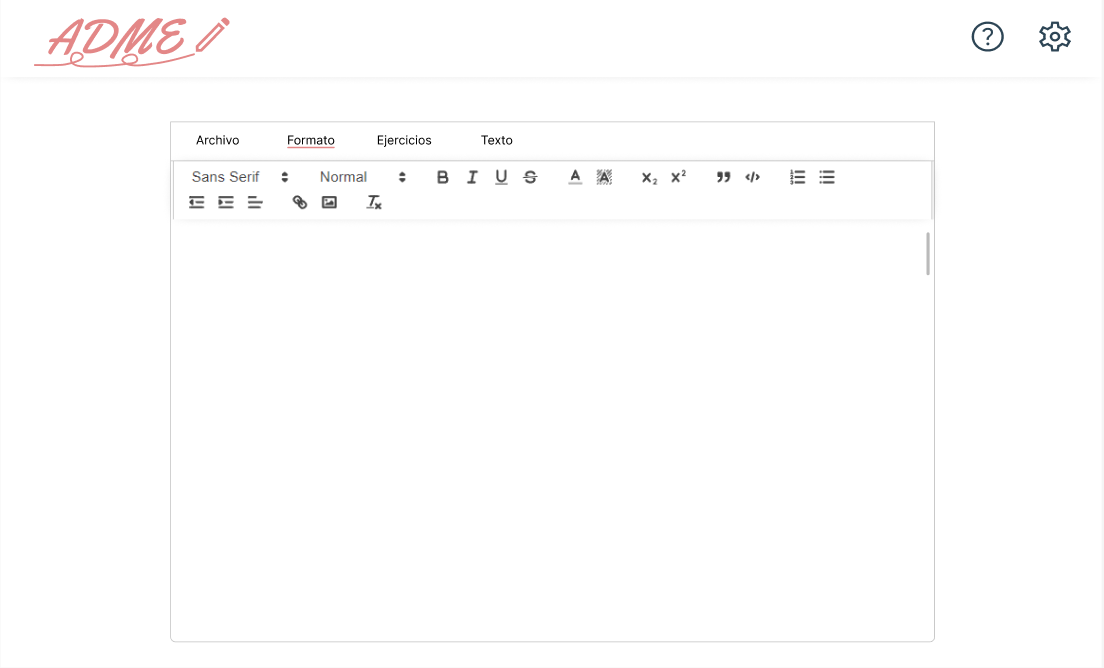
\includegraphics[width=15cm]{Diseño/Formato.PNG}
  \caption{Diseño de Formato pantalla de inicio.}
  \label{Forato}
\end{figure}


\begin{figure}[ht!]
  \centering
  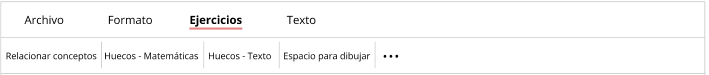
\includegraphics[width=15cm]{Diseño/Ejercicios.PNG}
  \caption{Diseño de Ejercicios pantalla de inicio.}
  \label{ejercicios}
\end{figure}


\begin{figure}[ht!]
  \centering
  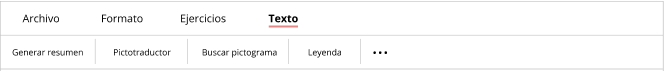
\includegraphics[width=15cm]{Diseño/Texto.PNG}
  \caption{Diseño de Texto pantalla de inicio.}
  \label{texto}
\end{figure}


\begin{figure}[ht!]
  \centering
  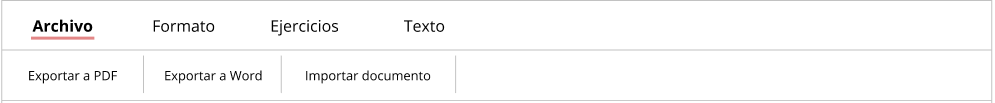
\includegraphics[width=15cm]{Diseño/Archivo.PNG}
  \caption{Diseño de Archivo pantalla de inicio.}
  \label{archivo}
\end{figure}

\subsubsection{Generar resumen}
El diseño de esta funcionalidad se muestra en la Figura \ref{resuemn} y se basa en el diseño de Álvaro Gómez, Figura \ref{fig:disenyoAlvaro03}. El usuario dispone de un panel en el que aparece el texto a resumir y el número de palabras que tendrá el resumen. Al pulsar el botón de resumir aparecerá en la parte inferior de la ventana modal una vista previa del resumen generado. El resultado de esta funcionalidad en el documento de trabajo se muestra en la Figura \ref{editable1}, en el ejercicio 3.

\begin{figure}[ht!]
  \centering
  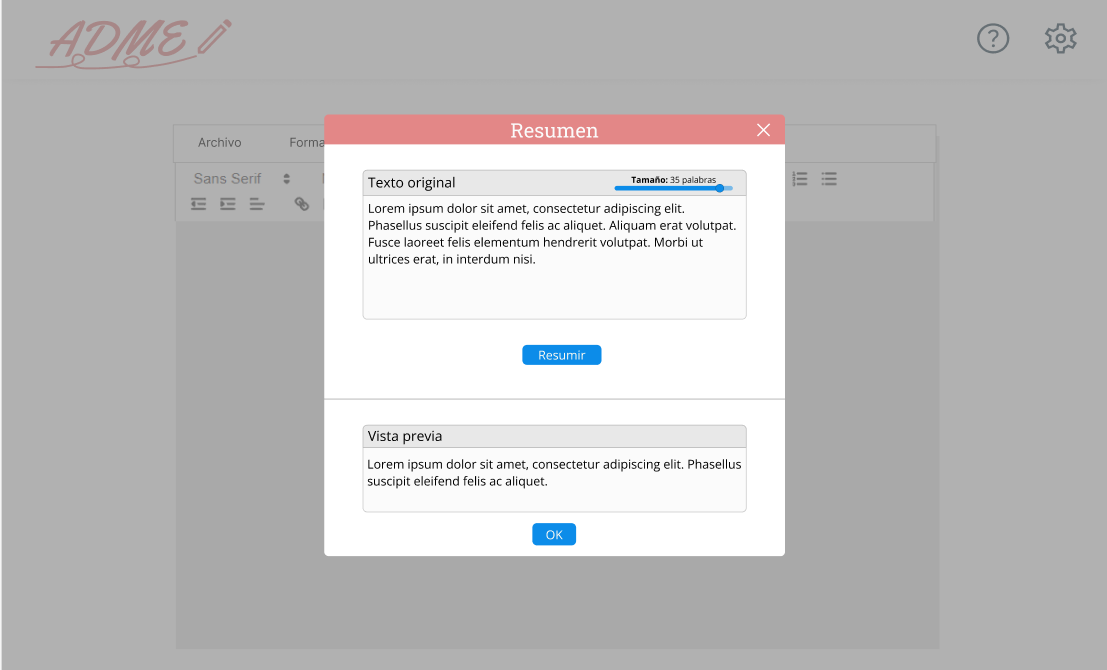
\includegraphics[width=15cm]{Diseño/Resumen.PNG}
  \caption{Diseño final generar resumen.}
  \label{resuemn}
\end{figure}

\subsubsection{Ejercicio de huecos}
El diseño de esta funcionalidad se muestra en la Figura \ref{definir_hueco}. Inicialmente habíamos pensado en que esta funcionalidad se pudiese hacer directamente sobre el documento de trabajo, pero al disponer de ventana modal y al ser complejo decidimos descartar dicha opción. En la ventana modal el usuario podrá escribir el texto. Una vez terminado le dará al botón de añadir huecos y pulsando sobre la palabra se pondrá un hueco y viceversa. Además, tiene la opción de elegir el tamaño de hueco, siendo pequeño, (5 caracteres), mediano, (12 caracteres) y grande, que es el por defecto, (23 caracteres). El resultado de esta funcionalidad en el documento de trabajo se muestra en la Figura \ref{editable3} en el ejercicio 3.

\begin{figure}[ht!]
  \centering
  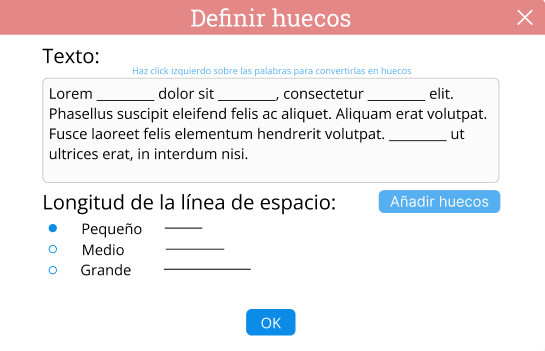
\includegraphics[width=0.7\textwidth]{Diseño/DefinirHuecos.PNG}
  \caption{Diseño final definir huecos.}
  \label{definir_hueco}
\end{figure}


\subsubsection{Sopa de letras}
El diseño de esta funcionalidad se muestra en la Figura \ref{sopaLetras}, se basa en el diseño de Alberto Rivas, (Figura \ref{Alberto16}). Inicialmente pensamos en tener dos botones, uno para añadir nuevas palabras, que se iba moviendo a la vez que se creaba una nueva palabra, y otro que se encontraba al lado de cada palabra para eliminarla, pero llegamos a la conclusión
de que era mejor que el botón de añadir palabras fuera fijo y no cambiara de posición cada vez que se añadiese una nueva palabra ya que esto le aportaría comodidad y facilidad de uso. Para ayudar al usuario a que sea más intuitivo decidimos incluir dos campos para que el usuario introduzca las filas y las columnas de la sopa de letras. También añadimos otro campo donde poner la palabra y al darle al botón de añadir la palabra se pondrá debajo de dicho campo junto a dos botones, uno de edición y otro para eliminar la palabra. Además, añadimos varias opciones para que el usuario elija cómo disponer las palabras en la sopa de letras (horizontal, vertical, diagonal y al revés). El resultado de esta funcionalidad en el documento de trabajo se muestra en la Figura \ref{editable2} en el ejercicio 5.

\begin{figure}[ht!]
  \centering
  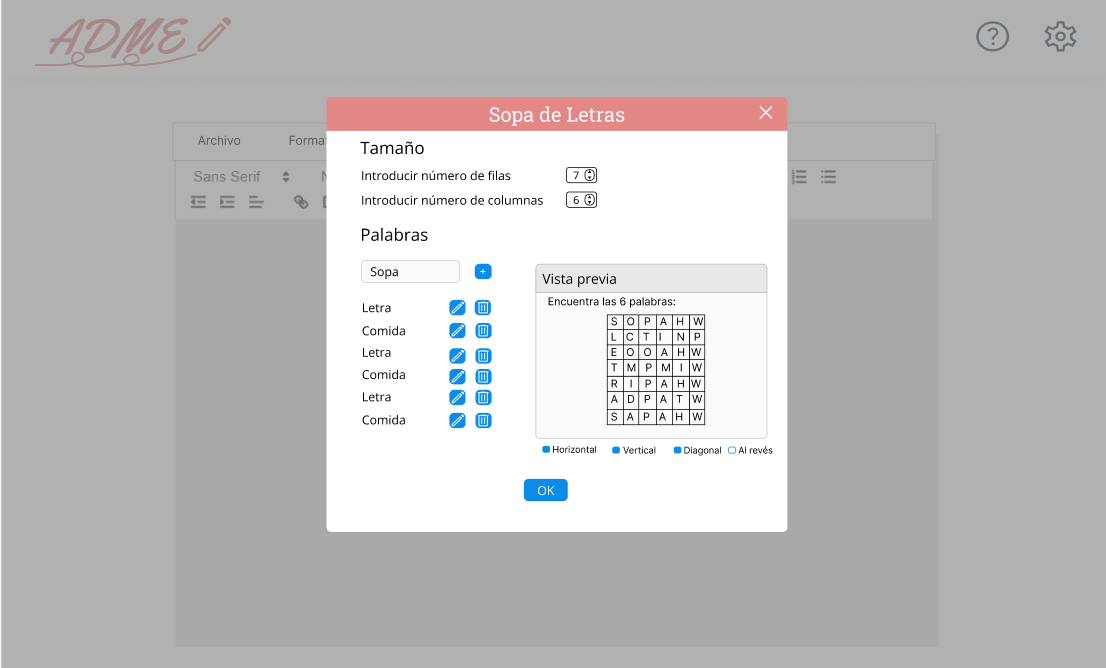
\includegraphics[width=0.7\textwidth]{Diseño/Sopa.PNG}
  \caption{Diseño final sopa de letras.}
  \label{sopaLetras}
\end{figure}

\begin{figure}[ht!]
  \centering
  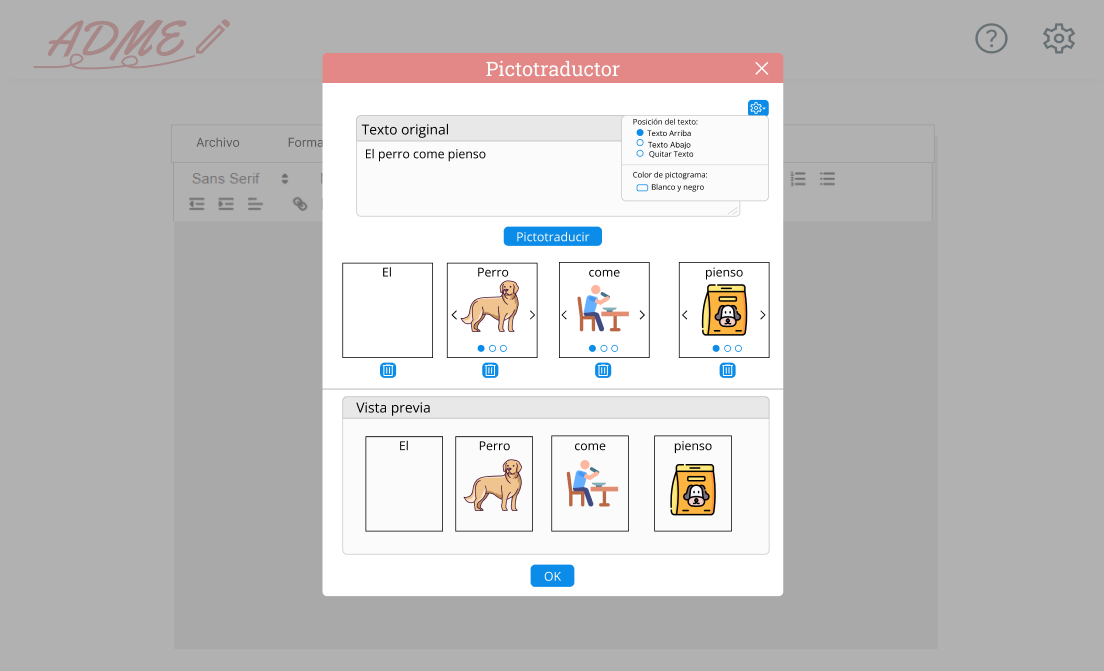
\includegraphics[width=0.7\textwidth]{Diseño/picto.PNG}
  \caption{Diseño final del pictotraductor.}
  \label{pictotraductor}
\end{figure}

\subsubsection{Pictotraductor}
El diseño de esta funcionalidad se muestra en la (Figura \ref{pictotraductor}), se basa en el diseño de Johan Salvatierra, Figura \ref{Johan7} y en la idea de Álvaro Gómez de que los pictogramas puedan cambiar en el caso de que haya varias opciones para una palabra. Inicialmente se pensó un diseño bastante simple en el que había un campo para añadir un texto y al pulsar sobre el botón de traducir a pictogramas se mostrasen los pictogramas. El problema de este diseño fue que no se tuvieron en cuenta varias opciones que necesita el usuario sobre el diseño de los pictogramas. Finalmente mantuvimos el campo de añadir el texto a traducir y el botón que te muestra los pictogramas con su respectiva palabra y añadimos un desplegable para escoger las opciones de posicionamiento de la palabra, color del pictograma y quitar la palabra asociada al pictograma. Por otra parte, cada pictograma tiene su propio botón de eliminar y unas flechas que permiten seleccionar otro de los pictogramas disponibles para la misma palabra del pictograma, en el caso de que haya varias opciones. El resultado de esta funcionalidad en el documento de trabajo se muestra en la Figura \ref{editable1} en el ejercicio 3.





\subsubsection{Ejercicio de flechas}
El diseño de esta funcionalidad se muestra en la Figura \ref{flechas} y se basa en el diseño de Dunia Namour, (Figura \ref{dunia4}). Inicialmente dábamos la opción de solo hacer dos columnas para relacionar con flechas, pero nos dimos cuenta de que el usuario debería poder elegir tantas columnas como desee. Tampoco tuvimos en cuenta que el usuario podría querer desordenar las columnas para que no tenga que pensar en el orden de las palabras. Con todo lo anterior creamos una ventana modal en la que se debe introducir el número filas y columnas, lo que genera tantas columnas vacías como haya indicado el usuario. Una vez que el usuario rellena dichas columnas tiene la opción de reordenar, la cual reordenaría cada columna. La ventana modal dispone de una vista previa en la cual se mostrará cómo quedaría el ejercicio de flechas, generándose automáticamente cada vez que el usuario realice un cambio en alguna de las columnas. El resultado de esta funcionalidad en el documento de trabajo se muestra en la Figura \ref{editable1} en el ejercicio 1.

\begin{figure}[ht!]
  \centering
  \includegraphics[width=0.7\textwidth]{Diseño/Flechas.PNG}
  \caption{Diseño final de ejercicios de fechas.}
  \label{flechas}
\end{figure}

\subsubsection{Ejercicio de desarrollo}
Partimos del diseño de AdaptaMaterialEscolar 1.0, dicho diseño no permitía al usuario cambiar el tipo de pauta ni elegir el interlineado. Todo lo mencionado anteriormente se ha añadido al nuevo diseño y también se ha incluido una vista previa que se genera automáticamente cada vez que se haga un cambio para que el usuario pueda visualizar cómo quedará el ejercicio. El diseño de esta funcionalidad se muestra en la Figura \ref{DesarrolloFinal}. El resultado de esta funcionalidad en el documento de trabajo se muestra en la Figura \ref{editable1} en el ejercicio 2.

\begin{figure}[ht!]
  \centering
  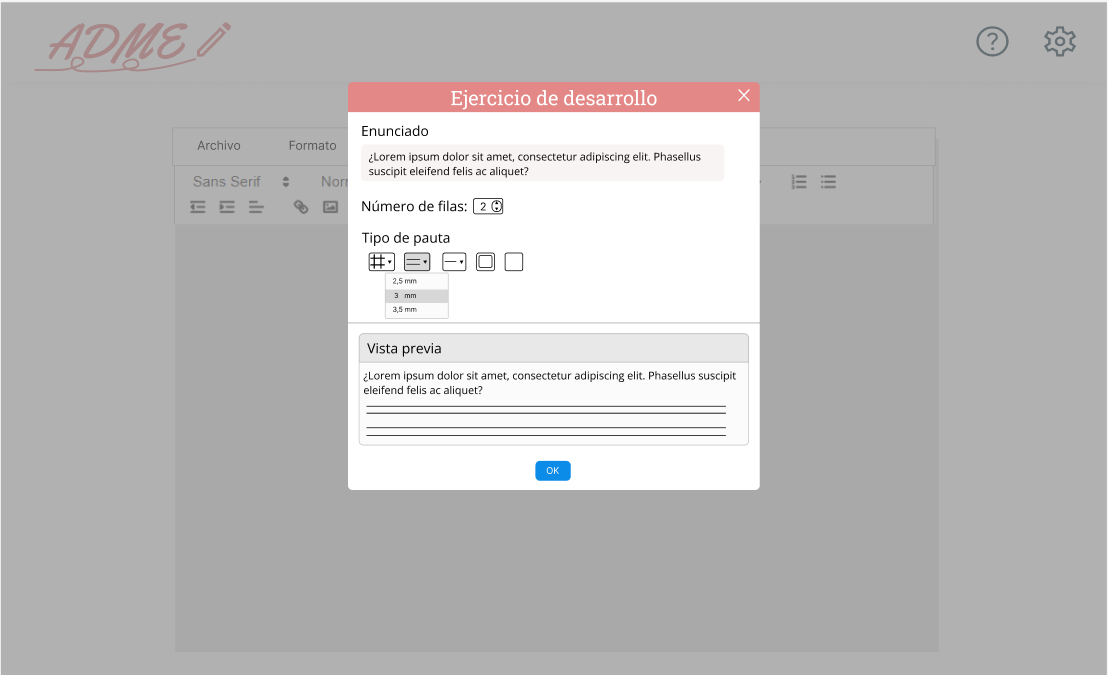
\includegraphics[width=0.7\textwidth]{Diseño/Desarollo.PNG}
  \caption{Diseño final de ejercicios de desarrollar.}
  \label{DesarrolloFinal}
\end{figure}


\begin{figure}[ht!]
  \centering
  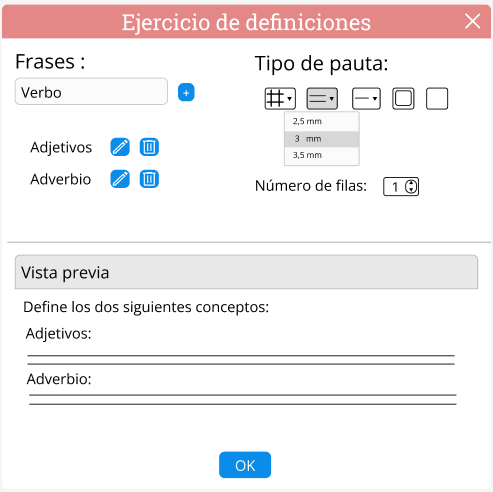
\includegraphics[width=0.7\textwidth]{Diseño/definiciones.PNG}
  \caption{Diseño final ejercicios de definiciones.}
  \label{defi}
\end{figure}

\subsubsection{Ejercicio de definiciones}
Partimos del diseño de AdaptaMaterialEscolar 1.0. Dicho diseño tenía los mismos problemas que el de ejercicios de desarrollo. El diseño final de esta funcionalidad se muestra en la Figura \ref{defi}. El resultado de esta funcionalidad en el documento de trabajo se muestra en la Figura \ref{editable2} en el ejercicio 3.


\subsubsection{Ejercicios de espacio para dibujar}
El diseño de esta funcionalidad se muestra en la Figura \ref{espaciosDibu}. En esta funcionalidad el usuario inicialmente tendrá que escribir el enunciado e indicar el espacio que desea dejar para dibujar. Además, incorpora una opción de recuadrar que hace un recuadro del tamaño indicado. El resultado de esta funcionalidad en el documento de trabajo se muestra en la Figura \ref{editable3} en el ejercicio 5.

\begin{figure}[ht!]
  \centering
  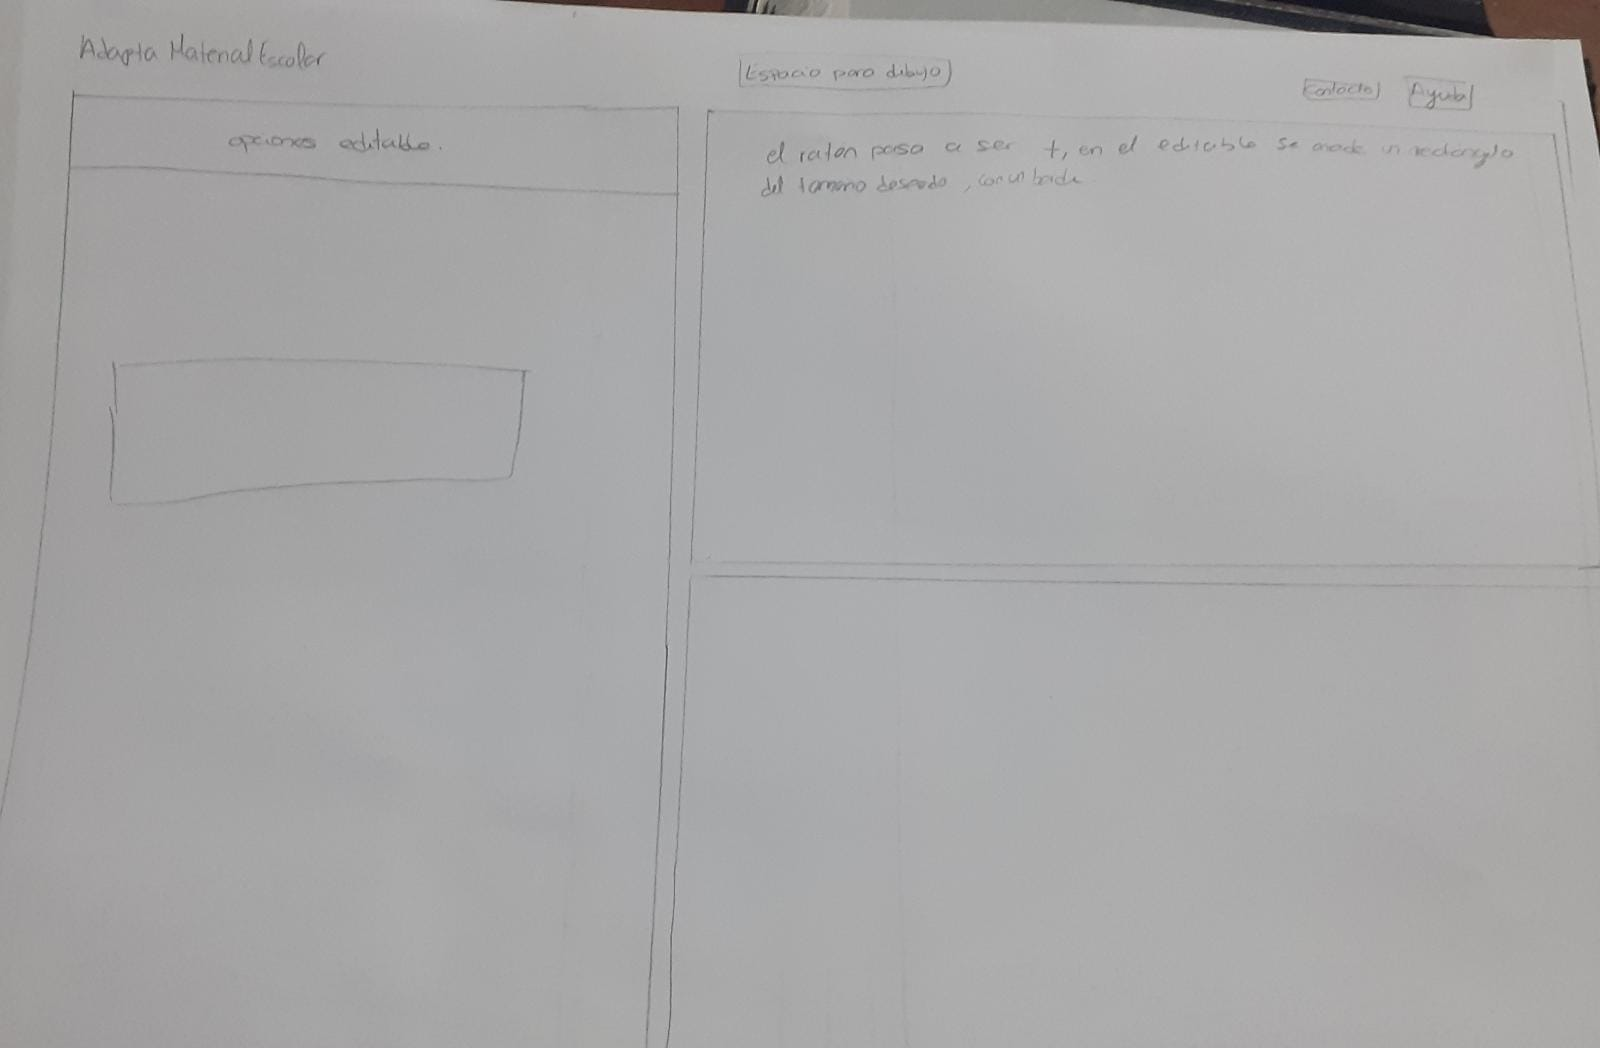
\includegraphics[width=0.7\textwidth]{Diseño/espacioDibu.PNG}
  \caption{Diseño final ejercicios espacios para dibujar.}
  \label{espaciosDibu}
\end{figure}

\subsubsection{Leyenda de colores}
El diseño final de esta funcionalidad se muestra en la Figura \ref{LeyendaColores} y para realizar esta funcionalidad no hemos basado en el diseño de todos los integrantes ya que son bastante parecidos. También hemos utilizado como referencia la funcionalidad de definir conceptos. En este caso cuando se añade un nuevo concepto también se ha de escoger un color para cada palabra. Además, se ha de incluir un título para la leyenda. La leyenda de color se situará en el documento de trabajo donde se encuentre el cursor y el usuario podrá ajustar su posicionamiento. El resultado de esta funcionalidad en el documento de trabajo se muestra en la Figura \ref{editable2} en el ejercicio 2.

\begin{figure}[ht!]
  \centering
  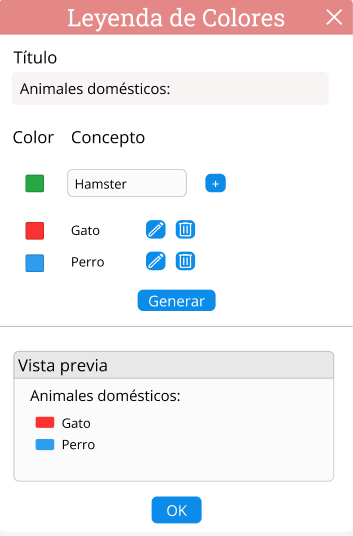
\includegraphics[width=0.7\textwidth]{Diseño/Leyenda.PNG}
  \caption{Diseño final leyenda de colores.}
  \label{LeyendaColores}
\end{figure}

\subsubsection{Ejercicio de matemáticas con huecos}
El diseño de esta funcionalidad se muestra en la Figura \ref{matesHueco} y para realizarla nos hemos basado en el diseño de Dunia Namour, Figura (\ref{dunia6}) y en la idea de Johan Salvatierra de que al pulsar la tecla \textit{espacio} se genere un hueco. Para introducir huecos en una fórmula matemática el usuario tendrá que darle a la barra espaciadora. Cuando termine de escribir la fórmula al darle al botón de \textit{OK} se introducirá en el documento de trabajo con un cuadrado vacío en cada hueco. El resultado de esta funcionalidad en el documento de trabajo se muestra en la Figura \ref{editable3} en el ejercicio 2.


\begin{figure}[ht!]
  \centering
  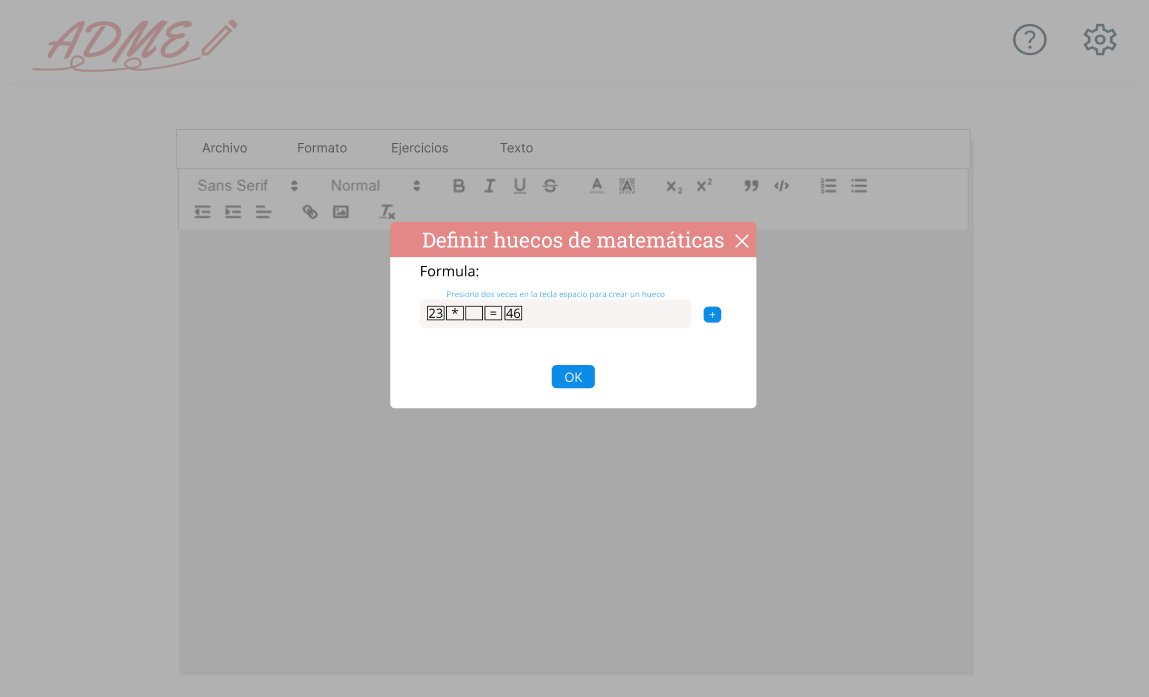
\includegraphics[width=0.7\textwidth]{Diseño/EjerMatesHuecos.PNG}
  \caption{Diseño final ejercicios de matemáticas con huecos.}
  \label{matesHueco}
\end{figure}

\subsubsection{Configuración general}
Debido a que gran parte de las funcionalidades tienen varias opciones hemos decidido crear una página de configuración para poder definir los ajustes por defecto. En esta página hay una configuración general por cada tipo de funcionalidad. El diseño de la configuración se muestra en la Figura \ref{configu}. Esta página surgió durante el brainstorming con las tutoras por la necesidad de tener ajustes por defecto.

\begin{figure}[ht!]
  \centering
  \includegraphics[width=15cm]{Diseño/configuracion.PNG}
  \caption{Diseño final de la configuración general.}
  \label{configu}
\end{figure}





\begin{figure}[ht!]
  \centering
  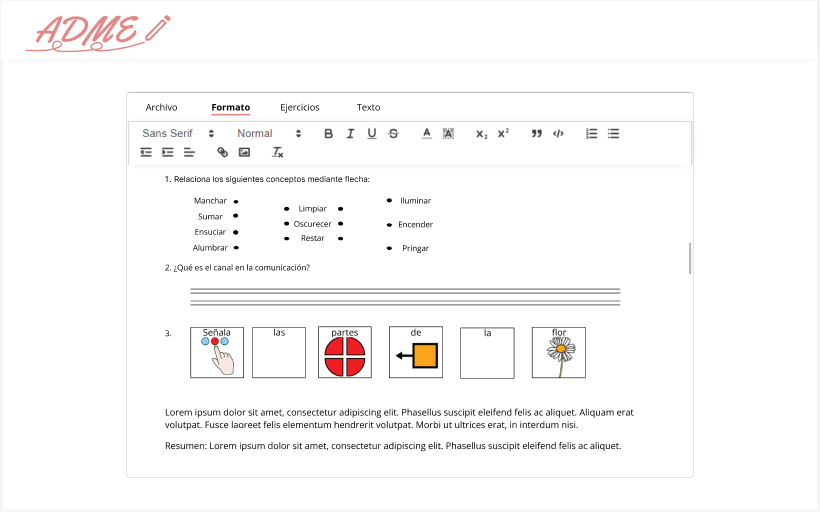
\includegraphics[width=15cm]{Diseño/Editable1.PNG}
  \caption{Resultado de las funcionalidades en el documento de trabajo.}
  \label{editable1}
\end{figure}


\begin{figure}[ht!]
  \centering
  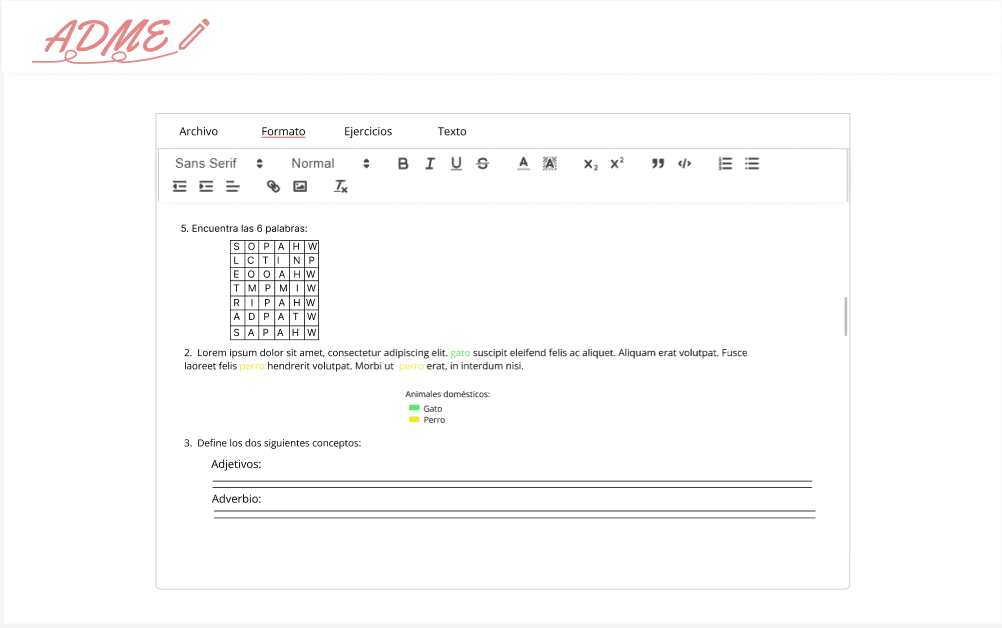
\includegraphics[width=15cm]{Diseño/editable2.PNG}
  \caption{Resultado de las funcionalidades en el documento de trabajo.}
  \label{editable2}
\end{figure}

\begin{figure}[ht!]
  \centering
  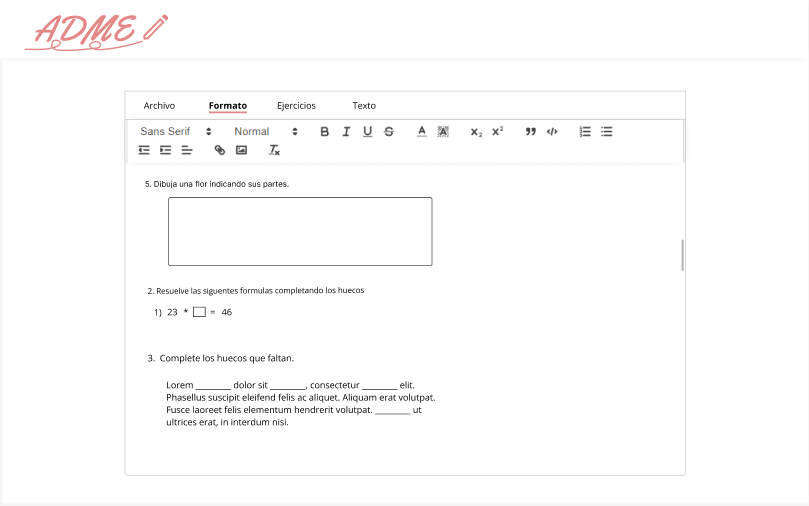
\includegraphics[width=15cm]{Diseño/Editable3.PNG}
  \caption{Resultado de las funcionalidades en el documento de trabajo.}
  \label{editable3}
\end{figure}

\section{Implementación}
% TODO: Introduccion
\subsection{Arquitectura}
En este TFG hemos decidido usar Slate, una biblioteca de JavaScript que se utiliza para construir editores de texto enriquecido. Lo hemos combinado con React lo que nos permite crear una aplicación basada en componentes que a largo plazo será más escalable. Ambas herramientas se apoyan en el patrón \textit{Composite}\footnote{\url{https://refactoring.guru/es/design-patterns/composite}} el cual permite generar un componente complejo mediante la anidación de componentes simples. Dicho patrón se encuentra integrado en Slate lo que nos facilita la configuración de este. En cuanto a la estructura interna de React ayuda a implementarlo, por nuestra parte lo hemos empleado para el diseño de los modales. Por otro lado, también hemos usado el patrón creacional \textit{Factory}\footnote{\url{https://refactoring.guru/es/design-patterns/factory-method}} que nos permite crear objetos sin tener que conocer los detalles de su creación, lo hemos usado para la creación de los modales y de las distintas barras de herramientas que se encuentran en el editor.

En cuanto a cómo se encuentran conectados Slate y React cabe mencionar que hemos creado un conjunto de funciones que hacen de intermediario entre los modales y el editor.

\begin{figure}[ht!]
  \begin{subfigure}{\textwidth}
    \centering
    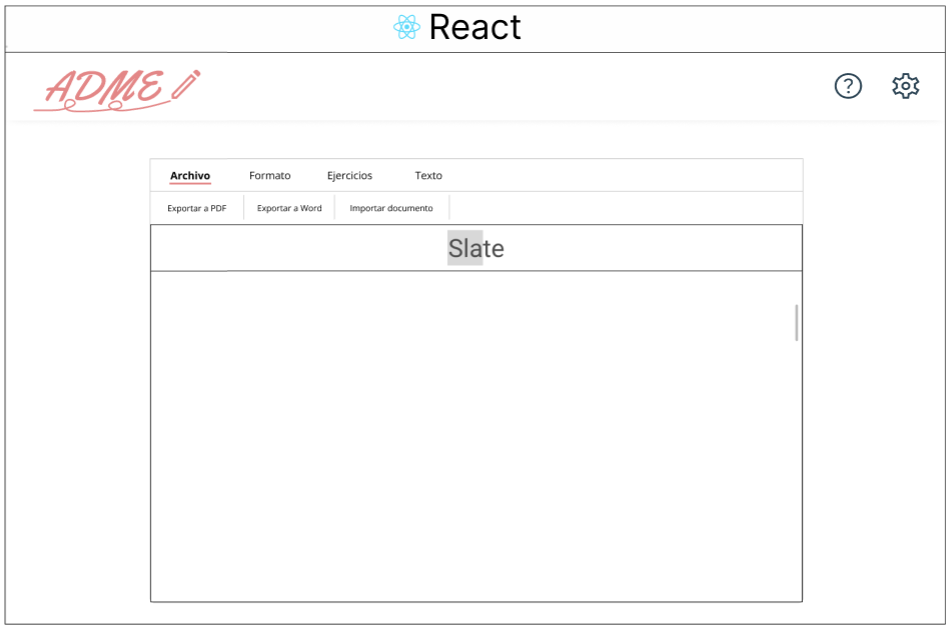
\includegraphics[width=0.7\textwidth]{Arquitectura/ArquitecturaPaginaInicio.png}
    \caption{Visión general de la página de inicio}
    \label{fig:arquitecturageneral1}
  \end{subfigure}

  \begin{subfigure}{\textwidth}
    \centering
    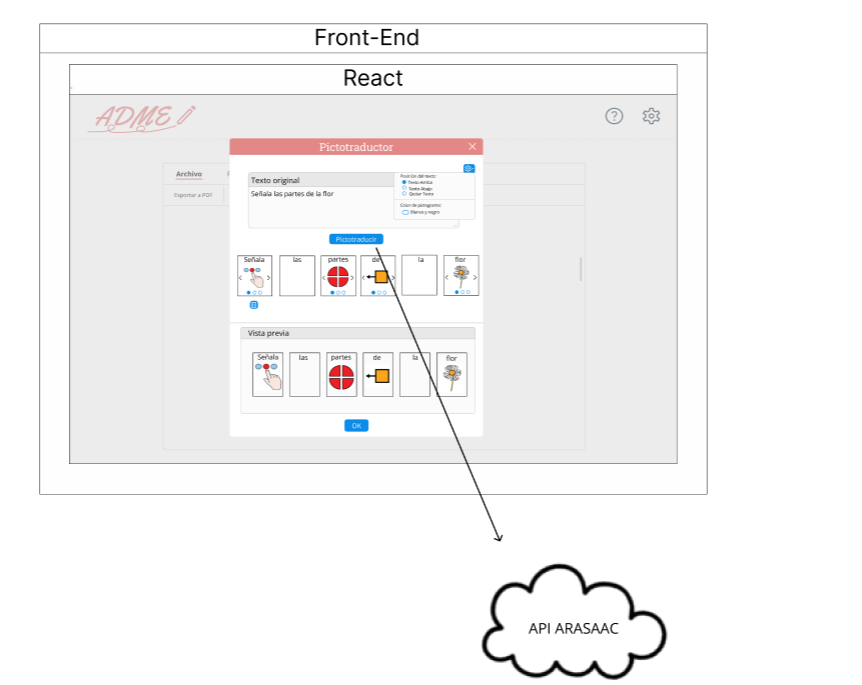
\includegraphics[width=0.7\textwidth]{Arquitectura/ArquitecturaPictoTraductor.png}
    \caption{Visión general de funcionalidad con conexión a API}
    \label{fig:arquitecturageneral2}
  \end{subfigure}
  \caption{Visión general de AdaptaMaterialEscolar 2.0}
  \label{fig:arquitecturageneral}
\end{figure}

\subsection{Funcionalidades}
A continuación se explican los detalles de implentación de las distintas funcionalidades que hemos rediseñado o creado de cero.
% TODO: Terminar introduccion

Para la explicación de las funcionalidades se pensó en realizar diagramas para facilitar la comprensión, pero tras debatirlo con las tutoras de este TFG y con Antonio Navarro Martín (profesor de Ingeniería y Modelado de Software), se llegó a la conclusión de que no hay aproximaciones para modelar React y JavaScript. Se comentó la posibilad de extender diagramas UML, utilizando la tesis de Humberto Cortés y Antonio Navarro\footnote{\url{https://www.worldscientific.com/doi/abs/10.1142/S0218194017500486}}, para poder modelar React y JavaScript, pero eso podría ser un TFG en sí mismo.